%%%%%%%%%%%%%%%%%%%%%%%%%%%%%%%%%%%%%%%%%%%%%%%%%%%%%%%%%%%%%%%%%%%%%%
% problem statement
\begin{statement}[
  problempoints=70,
  timelimit=1 second,
  memorylimit=512 MiB,
]{Lutrija}

\setlength\intextsep{-0.1cm}
\begin{wrapfigure}[7]{r}{0.22\textwidth}
\centering
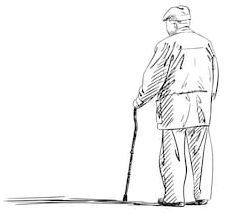
\includegraphics[width=0.22\textwidth]{img/vedran_kurdija.png}
\end{wrapfigure}

% \section

Grandpa Vedran is watching his favorite lottery show on TV in the hopes of
becoming an overnight millionaire. The lottery balls are spinning and bouncing
around before yielding the following draw: $2$, $5$, $7$, $11$, $19$, $23$ and
$31$.

Vedran sighs as he didn't guess a single one of those numbers. ``Looks like
I'm passed my prime...'', he thought to himself while turning off the old
TV. His vision is also getting worse, so he pressed the wrong button on the
remote control and switched to the COCI channel.

The host, Mr.\ Malnar, calmly spoke: ``Dear viewers, on the left side of the screen
I will show you a prime number $A$ and on the right side of the screen I will
show you a prime number $B$. The first person that calls in with an array of
prime numbers which starts with $A$, ends with $B$ and has a prime absolute
difference between each two neighbouring elements will receive a free trip
to IOI 2020 in Singapore.''


Old Vedran is reminiscing about his glory days of being a competitive programmer.
Unfortunately, he is rusty and is not able to solve the problem. Being
kindhearted, you decide to help Vedran win a trip to Singapore.

\textbf{Note:} A prime number is a positive integer greater than $1$ that is
only divisible by $1$ and itself.


%%%%%%%%%%%%%%%%%%%%%%%%%%%%%%%%%%%%%%%%%%%%%%%%%%%%%%%%%%%%%%%%%%%%%%
% Input
\subsection*{Input}
The first line contains two prime numbers $A$ and $B$
$(2 \le A, B \le 10^{14}, A \ne B)$ from the task description.

%%%%%%%%%%%%%%%%%%%%%%%%%%%%%%%%%%%%%%%%%%%%%%%%%%%%%%%%%%%%%%%%%%%%%%
% Output
\subsection*{Output}
If the task is impossible, i.e., there is no array satisfying the conditions
from task statement, simply output \texttt{-1} in a single line.

Otherwise, in the first line output the number of elements in the array and in
the second line output its elements separated by spaces. The size of array must
not be greater than $10^5$ and its elements must not be greater than $10^{15}$.
It is guaranteed that, if a solution exists, there is at least one satisfying
those bounds.

If there are multiple correct solutions, output any of them.

%%%%%%%%%%%%%%%%%%%%%%%%%%%%%%%%%%%%%%%%%%%%%%%%%%%%%%%%%%%%%%%%%%%%%%
% Scoring
\subsection*{Scoring}
In test cases worth a total of $14$ points, it will hold that if a solution
exists, there is at least one such that the number of elements in the resulting
array is not greater than $3$ and all of its elements are not greater than $1000$.

In test cases worth additional $28$ points, it will hold $2 \le A, B \le 1000$.

%%%%%%%%%%%%%%%%%%%%%%%%%%%%%%%%%%%%%%%%%%%%%%%%%%%%%%%%%%%%%%%%%%%%%%
% Examples
\subsection*{Examples}
\begin{tabularx}{\textwidth}{X'X'X}
\sampleinputs{test/lutrija.dummy.in.1}{test/lutrija.dummy.out.1} &
\sampleinputs{test/lutrija.dummy.in.2}{test/lutrija.dummy.out.2} &
\sampleinputs{test/lutrija.dummy.in.3}{test/lutrija.dummy.out.3}
\end{tabularx}

%%%%%%%%%%%%%%%%%%%%%%%%%%%%%%%%%%%%%%%%%%%%%%%%%%%%%%%%%%%%%%%%%%%%%%
% We're done
\end{statement}

%%% Local Variables:
%%% mode: latex
%%% mode: flyspell
%%% ispell-local-dictionary: "croatian"
%%% TeX-master: "../hio.tex"
%%% End:
